\documentclass{beamer}

\usepackage{agda}
\usepackage{apacite}
\usepackage{catchfilebetweentags}
\usepackage{changepage}
\usepackage{babel}

\usepackage{graphicx}

\usepackage[autostyle=true,french=guillemets,maxlevel=3]{csquotes}

\graphicspath{ {images/} }

\newcommand{\agda}[2]{\ExecuteMetaData[latex/#1.tex]{#2}}
 
\usetheme{Frankfurt}

\DeclareQuoteStyle{english}
  {\em}
	{\em}
	{\textquotedblleft\em}
	{\em\textquotedblright}

%Information to be included in the title page:
\title{Uma versão simplificada do Bitcoin, \\
  implementada em Agda}
\author[Guilherme, Flávio]{Guilherme Horta Alvares da Silva \\
  Orientador: Flávio Codeço Coelho}
\institute{Fundação Getulio Vargas}
\date{2019}

 
\begin{document}
 
\frame{\titlepage}

\begin{frame}
  \frametitle{Uma versão simplificada do Bitcoin, implementada em Agda}
\begin{itemize}
  \item Objetivo
  \item Justificativa
  \item Introdução
  \begin{itemize}
    \item Criptomoedas
    \item Agda
    \item Bugs em criptomoedas
  \end{itemize}
  \item Trabalho executado
  \item Próximos passos
  \item Referências Bibliográficas
\end{itemize}
\end{frame}

\section{Objetivo}

 \begin{frame}
\frametitle{Objetivo}
\begin{itemize}
  \item Programar uma criptomoeda (similar ao Bitcoin) em Agda, que é uma linguagem com tipos dependentes.
    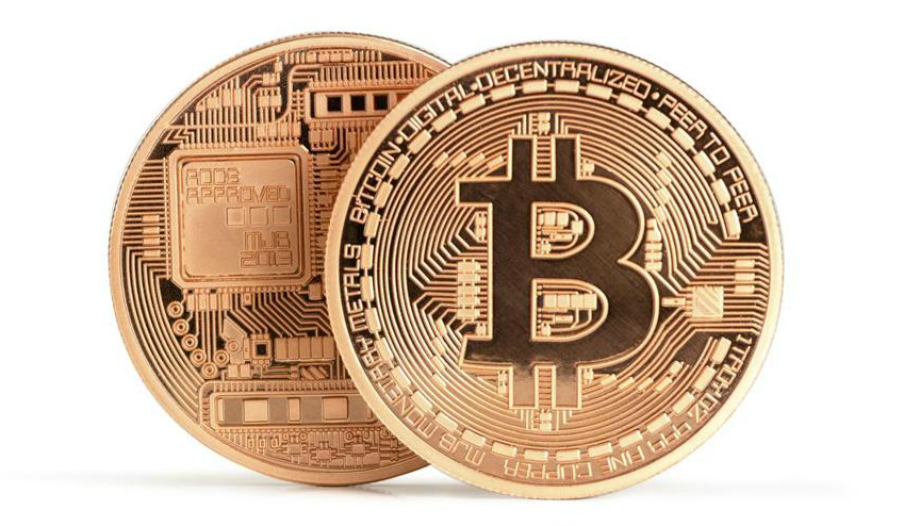
\includegraphics[width=8cm, height=5cm]{TwoBitcoins}
\end{itemize}
\end{frame}
 
\section{Justificativa}

\begin{frame}
\frametitle{Justificativa}
\begin{itemize}
    \item Programar um protocolo de criptomoedas livre de erros (bugs).
    \item Utilizar Agda permite, além da programação da criptomoeda, especificar como ela deve funcionar
      \cite{norell2008dependently}.
\end{itemize}
\end{frame}

\section{Linguagem Funcional}

\begin{frame}
\frametitle{Linguagem Funcional}
\begin{itemize}
  \item Em linguagens funcionais, toda função retorna o mesma saída para o mesma entrada.
  \item Em Agda, toda função é total e ela sempre termina.
\end{itemize}
\end{frame}

\begin{frame}
\frametitle{Efeitos Colaterais}
\begin{itemize}
  \item Para Agda ser utilizada como um programa, ela tem que lidar com o sistema operacional.
    Operação chamada de IO (Input Output).
  \item Várias pesquisas estão sendo feitas para minimizar os efeitos colaterais do IO.
  \item Lógica linear é usada para lidar com recursos, como abrir arquivos.
  \item Efeitos algébricos são utilizados para distinguir os diferentes tipos de efeitos
    relacionados ao sistema operacional.
\end{itemize}
\end{frame}

\begin{frame}
\frametitle{Efeitos Colaterais}
\begin{itemize}
  \item Frontend e backend de serviços estão sendo programados na mesma linguagem funcional
    para minimizar os efeitos colaterais.
  \item Haxl, usado no Facebook, é uma ferramenta que faz o cache das operações IO para
    fácil debug, log e teste.
  \item Facebook também faz Hot Swapping de forma funcional.
    Ou seja, ele não reinicia o processo para iniciar um novo.
    Algo que já era comum em Lisp.
  \item Sistemas distribuídos já estão sendo completamente descritos por meio de linguagens funcionais.
    Whatsapp utiliza Elixir como linguagem.
\end{itemize}
\end{frame}

\section{Industria}

\begin{frame}
  \frametitle{Beneficios}
  \begin{itemize}
    \item Por causa dos inúmeros benefícios das linguagens funcionais,
      elas estão sendo cada vez mais utilizadas na indústria.
    \item Garantem corretude de software.
      É de fácil reprodutibilidade, testabilidade e é mais fácil de debugar.
    \item Entretanto, elas são mais difíceis de serem aprendidas.
      Necessitam alto grau de abstração e
      é mais difícil de encontrar mão de obra.
  \end{itemize}
\end{frame}

\begin{frame}
  \frametitle{Empresas}
    
\includegraphics[width=2.5cm, height=2.5cm]{companies/Galois}
    
\includegraphics[width=2cm, height=2cm]{companies/barclays}
    
\includegraphics[width=2cm, height=2cm]{companies/fb}
    
\includegraphics[width=2cm, height=2cm]{companies/whatsapp}
    
\includegraphics[width=6cm, height=2cm]{companies/jane_street}
\end{frame}

\begin{frame}
  \frametitle{Criptomoedas}
    
\includegraphics[width=6cm, height=4cm]{crypto/cardano}
    
\includegraphics[width=4cm, height=4cm]{crypto/rchain}
    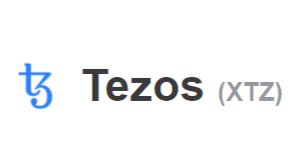
\includegraphics[width=6cm, height=4cm]{crypto/t3-tezos}
\end{frame}
 
\section{Agda}

 \begin{frame}{Agda}
 \begin{itemize}
    \item Linguagem funcional com sistema de tipos expressivos capazes de representar as especificações.
    \item Possibilita especificar e programar em um único lugar.
    \item O processo de verificação acontece no compilador.
 \end{itemize}
 \end{frame}
 
 \begin{frame}{Agda}
 \begin{itemize}
     \item A linguagem não possui \foreignquote{english}{Built-in} como em Python.
     \item Tipos como inteiros, ponto flutuantes, \foreignquote{english}{strings} e vetores devem ser definidos pelo próprio usuário.
     \item Tipos em Agda são uma generalização de tipos de dados algébricos encontrados em Haskell e ML.
 \end{itemize}
 \end{frame}

\section{Lambda Calculus}

 \begin{frame}{Identidade}
  \begin{itemize}
    \item Agda utiliza alguns conceitos do Lambda Calculus:
    \agda{lambdaCalculus}{Id}
    \agda{lambdaCalculus}{Id2}
  \end{itemize}
 \end{frame}
 
 \begin{frame}{Booleanos}
  \begin{itemize}
    \item Definição de booleanos:
      \agda{lambdaCalculus}{trueFalse}
  \end{itemize}
  \end{frame}

 \begin{frame}{Números naturais}
  \begin{itemize}
    \item Definição de números naturais:
      \agda{lambdaCalculus}{naturals}
  \end{itemize}
  \end{frame}

 \begin{frame}{Zero}
      \ExecuteMetaData[latex/lambdaCalculus.tex]{isZero}
  \end{frame}

 \begin{frame}{Soma}
      \agda{lambdaCalculus}{plus}
      \agda{lambdaCalculus}{onePone}
  \end{frame}

 \begin{frame}{Lista}
    \agda{lambdaCalculus}{list}
    \agda{lambdaCalculus}{sumList}
  \end{frame}

 \begin{frame}{Soma}
  \begin{itemize}
    \item Definição de tipos de soma:
      \agda{lambdaCalculus}{either}
  \end{itemize}
  \end{frame}

 \begin{frame}{Tipo soma}
    \agda{lambdaCalculus}{eitherRes}
  \end{frame}

 \begin{frame}{Tuplas}
  \begin{itemize}
    \item Definição de tupla:
      \agda{lambdaCalculus}{tuple}
      \agda{lambdaCalculus}{tupleExamples}
  \end{itemize}
  \end{frame}

 \begin{frame}{Adição de tuplas}
    \agda{lambdaCalculus}{tupleAdd}
  \end{frame}

\section{Agda}

\begin{frame}{Agda}
 \begin{itemize}
  \item Definição de números naturais em Agda:
  \item \agda{agdaExamples}{Nat}
 \end{itemize}
\end{frame}

\begin{frame}{Agda}
 \begin{itemize}
  \item Eliminação dos números naturais em Agda:
  \item \agda{agdaExamples}{NatElim}
 \end{itemize}
\end{frame}

\begin{frame}{Agda}
 \begin{itemize}
  \item Adição usando a recursão:
  \item \agda{agdaExamples}{sum}
 \end{itemize}
\end{frame}

\begin{frame}{Agda}
 \begin{itemize}
  \item Adição usando a eliminação dos naturais:
  \item \agda{agdaExamples}{sumElim}
 \end{itemize}
\end{frame}

\begin{frame}{Agda}
 \begin{itemize}
  \item Eliminação do tipo vazio:
  \item \agda{agdaExamples}{botType}
 \end{itemize}
\end{frame}

\begin{frame}{Agda}
  \agda{agdaExamples}{eitherType}
\end{frame}

\begin{frame}{Agda}
 \begin{itemize}
  \item Tipo booleano em Agda:
  \item \agda{agdaExamples}{boolType}
 \end{itemize}
\end{frame}

\begin{frame}{Agda}
 \begin{itemize}
  \item Usando tipos booleanos em casos:
  \item \agda{agdaExamples}{ifThenElse}
 \end{itemize}
\end{frame}

\begin{frame}{Agda}
 \begin{itemize}
  \item Eliminação do para todo:
  \item \agda{agdaExamples}{piType}
 \end{itemize}
\end{frame}

\begin{frame}{Agda}
 \begin{itemize}
  \item Tipo soma:
  \item \agda{agdaExamples}{sumType}
 \end{itemize}
\end{frame}

\begin{frame}{Agda}
 \begin{itemize}
  \item Tipo vetor:
  \item \agda{agdaExamples}{vector}
 \end{itemize}
\end{frame}

\begin{frame}{Agda}
 \begin{itemize}
  \item Encontrando primeiro elemento do vetor:
  \item \agda{agdaExamples}{vecHead}
 \end{itemize}
\end{frame}

\begin{frame}{Agda}
 \begin{itemize}
  \item Tipos booleanos:
  \item \agda{agdaExamples}{dataConstructor}
 \end{itemize}
\end{frame}

\begin{frame}{Agda}
 \begin{itemize}
  \item Funções que retornam tipo:
  \item \agda{agdaExamples}{patternMatch}
 \end{itemize}
\end{frame}

\begin{frame}{Agda}
 \begin{itemize}
  \item Utilizando records:
  \item \agda{agdaExamples}{record}
 \end{itemize}
\end{frame}

\begin{frame}{Agda}
 \begin{itemize}
  \item Demonstrando que elementos podem ser encontrados:
  \item \agda{agdaExamples}{wf}
 \end{itemize}
\end{frame}

\begin{frame}{Agda}
 \begin{itemize}
  \item Definindo o que é uma categoria:
  \item \agda{agdaExamples}{category}
 \end{itemize}
\end{frame}

\section{Criptomoedas}

\begin{frame}
  \frametitle{Definição}
\begin{itemize}
    \item Uma criptomoeda é um meio de troca descentralizado que se utiliza da tecnologia
      de blockchain e da criptografia para assegurar a validade das transações e a criação de novas unidades da moeda.
    \item O bitcoin é considerado a primeira moeda digital mundial descentralizada,
      constituindo um sistema econômico alternativo (\foreignquote{english}{peer-to-peer electronic cash system})
      e responsável pelo ressurgimento do sistema bancário livre.
      \cite{nakamoto2008bitcoin}
    \item O Bitcoin permite transações financeiras sem intermediários,
      mas verificadas por todos usuários (nodos da rede).
      Essas transações são gravadas em um banco de dados distribuídos (uma rede descentralizada),
      chamado de \foreignquote{english}{blockchain}.
    \end{itemize}
\end{frame}

\section{Bug}

 \begin{frame}
   \frametitle{Maleabilidade de transacao}
\begin{itemize}
  \item Nesse tipo de bug, é possível alterar o hash da transação depois que ela foi enviada.
  \item Todos os dados para calcular o hash não eram previamente calculados. Assim, o minerador poderia alterar o hash da transação.
  \item O ataque consistiria de um usuário enviar uma transação e ela não ser confirmada pelo sistema.
    Logo em seguida, esse mesmo usuário enviaria uma outra transação. Dessa forma, ele faria duas transações com a mesma moeda.
  \item Esse tipo de BUG pode ser evitado usando tipos dependentes.
    Colocando como característica da transação, o fato de seu ID ser único.
\end{itemize}
\end{frame}

\begin{frame}
  \frametitle{DAO Bug}
  \begin{itemize}
    \item \foreignquote{english}{Bug} que aconteceu em um cripto-contrato da rede Ethereum com um prejuízo de mais do que 250 milhões de dólares.
      \cite{wood2014ethereum}
    \item No cripto-contrato, existia uma função recursiva que não terminava.
      Ou seja, o usuário enviava uma quantidade de ethereum,
      depois acontecia um \foreignquote{english}{loop} infinito e só depois era feito a atualização do seu balanço.
    \item Em Agda, esse tipo de bug seria evitado, pois é necessário provar que a função termina.
      Logo, \foreignquote{english}{loops} infinitos não são possíveis em Agda.
  \end{itemize}
\end{frame}

\section{Criptomoedas}
\begin{frame}
  \frametitle{Função hash}
  \begin{itemize}
    \item Uma função hash é uma função que serve para comprimir dados grandes, como um vídeo,
      em um número pequeno.
      De forma que dois arquivos diferentes sempre terão hashes diferentes (injetividade).
    \item Pelo princípio da casa dos pombos, isso é impossível.
      Porém, nunca foi encontrado nenhum dois arquivos que possuem o mesmo hash.
    \item O Google encontrou dois arquivos que possuíam o mesmo hash no SHA-1.
      Logo em seguida, essa função hash parou de ser usada.
  \end{itemize}
\end{frame}

\begin{frame}
  \frametitle{Funções criptográficas}
  \begin{itemize}
    \item No bitcoin, existe a chave privada e a pública.
    \item A chave privada serve para assinar a transação.
    \item A chave pública, derivada da chave pública,
      serve para demonstrar que você é o dono da chave privada.
    \item Essas funções utilizam como base a função hash SHA-256.
  \end{itemize}
\end{frame}


\begin{frame}
  \frametitle{Funções criptográficas}
    \agda{Crypto}{cryptoPostulates}
\end{frame}

\begin{frame}
  \frametitle{Conta do bitcoin}
    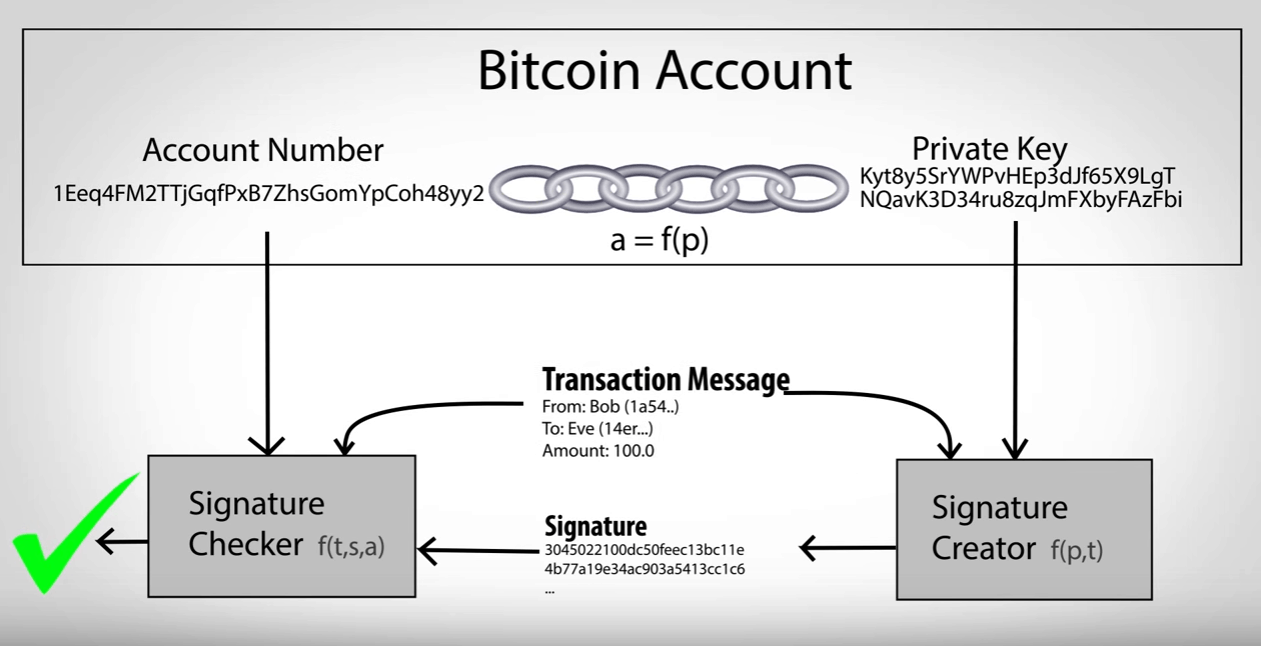
\includegraphics[width=11cm, height=7cm]{privatekey}
\end{frame}

\begin{frame}
  \frametitle{Transações}
  \begin{itemize}
    \item A partir de transações, é possível enviar bitcoins de uma conta para outra.
    \item Transações são como um cheque. O indivíduo especifica um valor e assina a transação.
    \item Na transação do bitcoin, deve ser especificado as transações anteriormente não gastas.
      No caso da transação do minerador, isso não deve ser especificado.
      Além do mais, deve ser especificado quem deve receber o dinheiro dessas transações e
      também a transação deve ter uma assinatura gerada a partir da chave privada comprovando
      que o usuário da chave pública aceitou fazer aquela transação.
  \end{itemize}
\end{frame}

\begin{frame}
  \frametitle{Transações}
  \agda{Transactions}{TXSigned}
\end{frame}

\begin{frame}
  \frametitle{Modelo de transações}
  \begin{itemize}
    \item O Bitcoin utiliza o modelo de transações não gastas enquanto o Ethereum utiliza
      o tradicional modelo bancário.
    \item No modelo bancario, cada conta possui um saldo.
      E em toda transação, o saldo da pessoa que enviou é subtraído e o saldo da pessoa que
      recebeu é incrementado.
    \item Nesse modelo tradicional, é fácil verificar o saldo de cada um.
      Porém é difícil saber como se chegou nesse estado final.
  \end{itemize}
\end{frame}

\begin{frame}
  \frametitle{Modelo de transações não gastas}
  \begin{itemize}
    \item No modelo de transações não gastas, toda transação é adicionada à árvore de transações.
    \item Para saber o saldo de uma conta é necessário olhar todas as transações não gastas
      foram enviadas para essa conta.
    \item Para transacionar a moeda é necessário utilizar como entrada as saídas das outras
      transações não gastas.
  \end{itemize}
\end{frame}

\begin{frame}
  \frametitle{Bitcoin UTXO}
    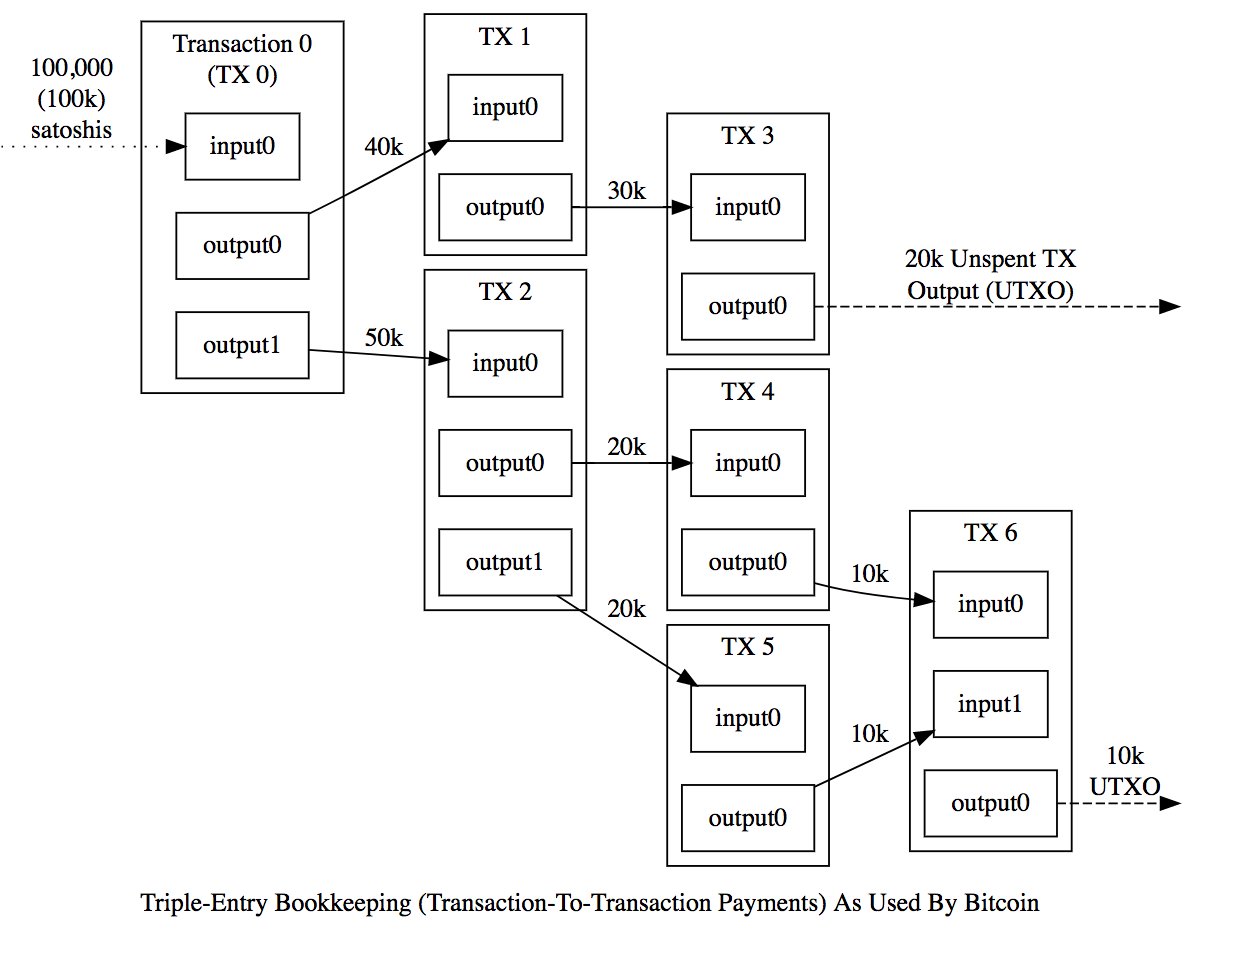
\includegraphics[width=11cm, height=7cm]{utxo}
\end{frame}

\begin{frame}
  \frametitle{Árvores de transação}
  \begin{itemize}
    \item A ideia da árvore de transação é reunir todas as transações em uma árvore.
    \item Dessa forma, é possível sintetizar a informação de todas as transações
      calculando apenas o hash dela.
    \item Com a propriedade da injetividade do hash, é possível verificar que duas árvores
      são iguais em complexidade de tempo constante.
  \end{itemize}
\end{frame}

\begin{frame}
  \frametitle{Árvore de transação}
    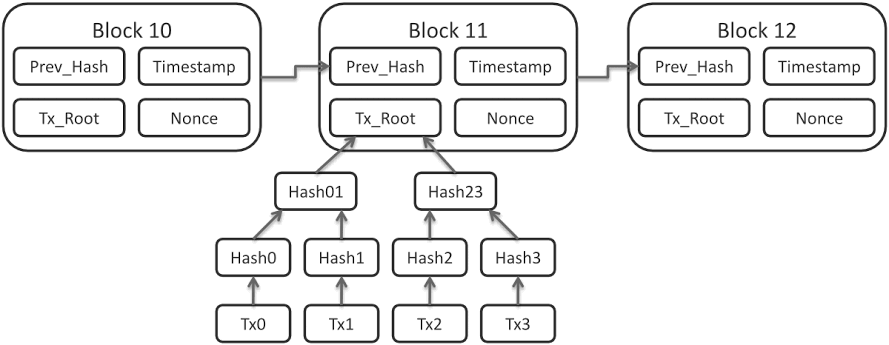
\includegraphics[width=10cm, height=5cm]{blockchain}
\end{frame}

\begin{frame}
  \begin{scriptsize} \agda{TXTree}{TXTree} \end{scriptsize}
\end{frame}

\begin{frame}
  \begin{scriptsize} \agda{TXTree}{TX} \end{scriptsize}
\end{frame}

\begin{frame}
  \frametitle{Blocos e cadeia de blocos}
  \begin{itemize}
    \item As transações são incorporadas em blocos aonde são armazenadas.
    \item No Bitcoin, existe uma cadeia de bloco chamada de blockchain.
      O primeiro bloco é chamado de \foreignquote{english}{genesis block} e
      a cada 10 minutos em média, um novo bloco é incorporado a essa cadeia de blocos.
    \item Existe um limite de transações que cada bloco pode possuir (no Bitcoin, é 10 MB de dados).
      Por isso, é importante pagar uma taxa de transação para que essa transação seja incluída na
      cadeia de blocos.
    \item Se existirem duas blockchains em computadores diferentes, é considerado
      como a cadeia de blocos válida aquela que tiver mais blocos.
  \end{itemize}
\end{frame}

\begin{frame}
\frametitle{Blockchain}
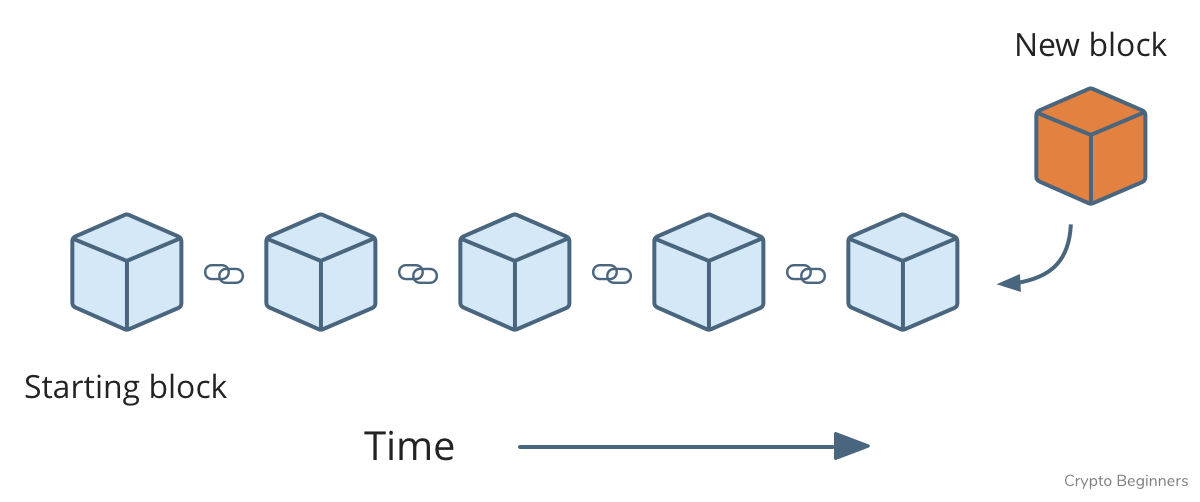
\includegraphics[width=11cm, height=8cm]{blockchain1}
\end{frame}

\begin{frame}
\frametitle{Blockchain}
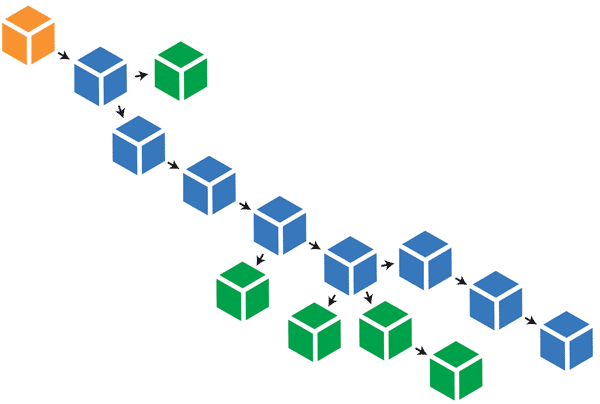
\includegraphics[width=11cm, height=8cm]{blockchain2}
\end{frame}

\begin{frame}
  \frametitle{Mineração}
  \begin{itemize}
    \item As transações são incorporadas em blocos aonde são armazenadas.
    \item No Bitcoin, existe uma cadeia de bloco chamada de blockchain.
      O primeiro bloco é chamado de \foreignquote{english}{genesis block} e
      a cada 10 minutos em média, um novo bloco é incorporado a essa cadeia de blocos.
    \item Todo bloco possui um problema criptográfico a ser resolvido. Ou seja,
      é preciso calcular um valor \foreignquote{english}{nounce} tal que o hash do bloco
      seja menor que o um valor especificado.
    \item Esse valor especificado é calculado a partir da média dos últimos 2016 blocos (2 semanas)
      para que a média de mineração de blocos seja de 2 semanas.
  \end{itemize}
\end{frame}

\begin{frame}
  \begin{scriptsize} \agda{Blockchain}{block} \end{scriptsize}
\end{frame}


\section{Próximos Passos}

\begin{frame}{Ressalvas}
  \begin{itemize}
    \item Nesse trabalho, todas as especificações foram colocadas nos tipos.
    \item Em outros trabalhos, a abordagem pode ser diferente.
      Ou seja, sem nenhuma informação nos tipos e todas as provas feitas de forma separada.
    \item Essa abordagem não foi escolhida, pois é muito mais simples de entender o código
      quando os tipos são mais expressivos.
  \end{itemize}
\end{frame}

\begin{frame}{Detalhes do que falta}
  \begin{itemize}
    \item Fazer o cálculo do hash do bloco e o campo nounce do bloco.
    \item Mudar o protocolo para receber o bloco inteiro ao invés de transações individuais.
    \item Adicionar o caso de existir uma blockchain de tamanho maior que a do que a do servidor.
  \end{itemize}
\end{frame}

\begin{frame}{Partes mais complexas de adicionar}
  \begin{itemize}
    \item Fazer a modelagem formal da cadeia de blocos como um sistema distribuído.
    \item Criar código do cliente para interagir com os nós.
    \item Especificar o protocolo entre cliente e nó e entre nó com nó.
      Entretanto, a parte mais difícil já foi codificada, que é adicionar as provas
      ao dado puro que o cliente envia.
    \item Adicionar uma linguagem de script na criptomoeda.
  \end{itemize}
\end{frame}

\begin{frame}{Outras ideias}
  \begin{itemize}
    \item Melhorar o sistema de tipos.
    Por enquanto, está se usando tipos dependentes, mas seria interessante utilizar tipos lineares
    para evitar o coletor de lixo ou usar \foreignquote{english}{Cubical Type Theory} por ser mais expressivo.
  \item
    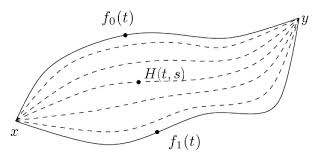
\includegraphics[width=5cm, height=3cm]{homotopy}
    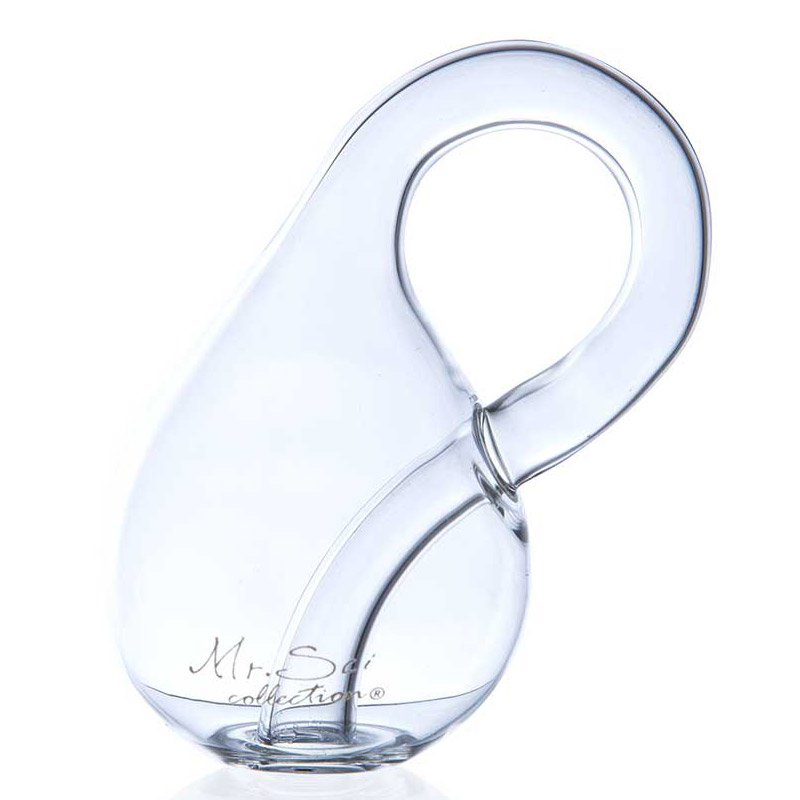
\includegraphics[width=4cm, height=4cm]{kleinBottle}
  \end{itemize}
\end{frame}

\begin{frame}{Outras ideias}
  \begin{itemize}
  \item  Utilizar outros provadores de teoremas.
    O Lean 4 e CoQ possuem táticas, algo que Agda não possui.
    O Idris 2 possui tipos lineares. 
  \item Utilizar teorias das categorias para deixar o código mais abstrato e conciso.
    Além de poder utilizar as bibliotecas já implementadas da linguagem.
  \item Utilizar bibliotecas para facilitar a transferência de mensagens entre nós diferentes.
    Cloud Haskell já facilita bastante esse processo.
  \end{itemize}
\end{frame}


\section{Bibliografia}

\begin{frame}{Referências Bibliográficas}
  \bibliographystyle{apacite}
  \bibliography{References}
\end{frame}

\end{document}
